% ------------------------------------------------------------------------------
% Chapter 1 : Introduction
% ------------------------------------------------------------------------------
% parameters setting
\setlength{\parindent}{4em}
\setlength{\parskip}{1em}

This thesis evaluates approach of estimating the performance of software workload on embedded hardware using machine learning. This is achieved by researching different available techniques, approaches and tools to evaluate performance of software on embedded hardware processor. This work is an attempt to represent the relevant features and highlighting various factors in existing methodology. 


\par Now a days electronic systems are widely used in automotive industry. These electronic systems provide better control than mechanical control with use of the software. These systems are used in commercial vehicles, trucks, motorcycles, forklifts, tractors, excavators and many more automobiles. And these electronic systems provide better control to and collect information from automobiles. These systems consist of electronic components such as processors, sensors, actuators, electrical components, electrical circuits, communication devices, power supply units and others. 

\par Electronic systems provide control operations in different domains of vehicles such as powertrain, chassis, passive safety, body/comfort, multimedia/telematics and man-machine interface which consist functionality like engine management, gearbox control, anti-locking system, electronic stability program, airbag control, navigation,instrument panel and many more. All these domains are connected and communicate to each other through on board electronic bus systems techniques such as Controller area network(CAN), Media oriented systems transport(MOST), etc.

\par In automotive electronics systems, Electronic control unit(ECU), is embedded system provides control to one or more electrical systems or subsystems in vehicles. ECU consist processors, interface for inputs and outputs, memory, communication links and many more. All sub domains discussed above consist one or more ECU as electronic system. Now a days upto 80 ECUs are used in modern cars. Development of ECU involves hardware and software to execute tasks for defined module. ECUs are programmable and can be reprogrammed according to functionality and requirements. Now a days, ECUs have more computing powers in single processor. Modern days processors provide higher computing powers typically upto 64 bit processing and operating frequency in gigahertz. Following figure \ref{fig:ecu} illustrate the ECUs used in various domains of a vehicle. Automotive electronic control unit market predicted to reach upto \$55.97 billion by 2024. Around 40\% of revenue in automotive industry is from automotive electronics. This is because most of vehicles are software driven[ref].

\begin{figure}[h!]
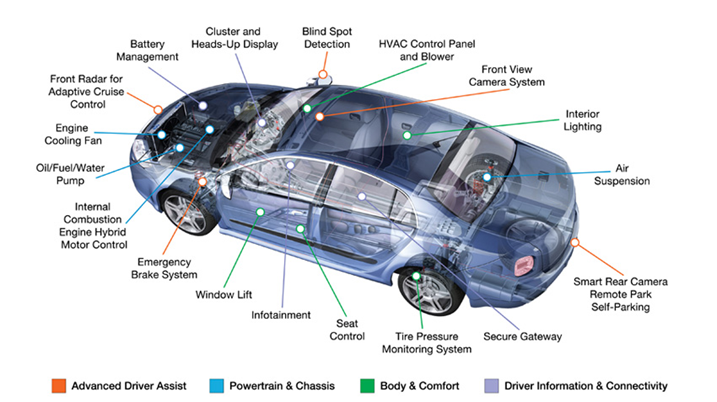
\includegraphics[width=12cm, height=8cm]{./images/ecus_in_car}
\centering
\caption{Number of ECUs are used in different domains of single vehicle}
\label{fig:ecu}
\end{figure}

\par Software is an integral part of embedded system in automotive domain. Software is running on microprocessors/microcontrollers provides the control mechanism. It is brain behind the every action taken in embedded systems. In current era, software is backbone for advanced features used in automobiles such as advance driving assistant systems have anti-breaking systems(ABS), electronic stability program(ESP), parking assistance system and many more. It also perform measure role in safety critical system used in automobile. As software plays important role in embedded systems then performance of software is also essential. Performance of software in application of safety critical systems is not only needed to be correct but also should have quick repose time. So performance of any software running on embedded hardware need to be evaluated before integrate with real hardware and used in application. 

\par Software performance is not only about how fast it can handle large numbers but it is also about memory management, networks, cores, architectures. Some algorithms looks good on paper but they perform poorly on hardware. Being able to manage the performance of software requires well understanding of hardware architecture, operating systems and runtime libraries[ref- lemire.me].  As mentioned above, modern cars have more than 70 ECUs per vehicle.  Following figure \ref{fig:num_ecu} shows increase in the number of ECUs year by year in automotive industry. Each ECU has number of functionalities to perform. Year by year number of ECUs per vehicle are increasing and ability to perform functionalities per ECU is also increasing. According to Moore's law, number of transistors on integrated circuits doubles approximately every two years. This advancement in capabilities of a ECU is due to growth in technology of semiconductor manufacturing as well as demand of software driven vehicles.  

\par Each ECU in vehicle has it's own software stack to control the operations, diagnostics, monitoring the network, reading the sensor values, to operate the actuators and many operations. In demand of software driven vehicles software performs the crucial part in it. Whether it is safety critical systems, powertrain system, advance driving assistance systems, multimedia systems in vehicle. All these systems have their own ECUs which controlled by software. In world of competition, each original equipment manufacturers and suppliers wants to stay ahead of each other and they are coming with new features and technology in the automotive industry. In current trade of automotive industry and future of automotive industry, interest in software driven vehicle is increasing and it is expecting improvement in hardware which can deliver the adequate performance of software. Software is playing the vital role of performance of vehicle as well as in automotive industry.

\begin{figure}[h!]
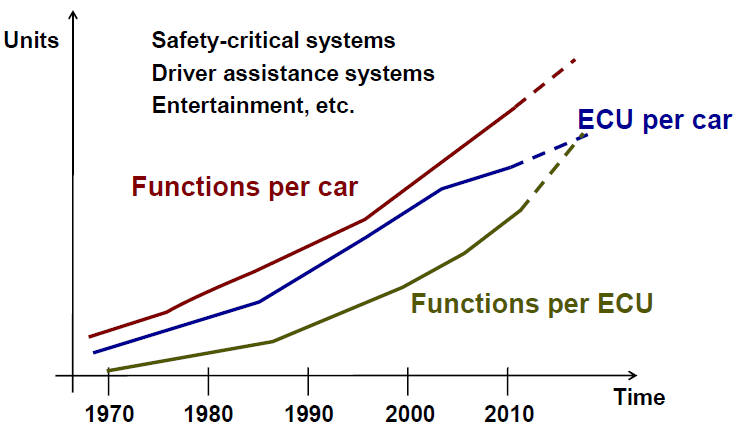
\includegraphics[width=12cm, height=8cm]{./images/ecu_per_year}
\centering
\caption{Trends in automotive systems}
\label{fig:num_ecu}
\end{figure}


\section{Purpose of the Thesis Work}
In initial phase of the thesis work, we discussed the problems behind the product development with sequential method and effect of the market pressure to release the product. Also tools available in market to evaluate the performance of software.

\subsection{Sequential development}
In automotive industry, sequential product development model is used widely to develop a product. V-model is one the broadly used process to develop a product. V model is also known as verification and validation model and processing is performed in V-shape. You can see in following figure \ref{fig:v-model} the V-model design.

\begin{figure}[h!]
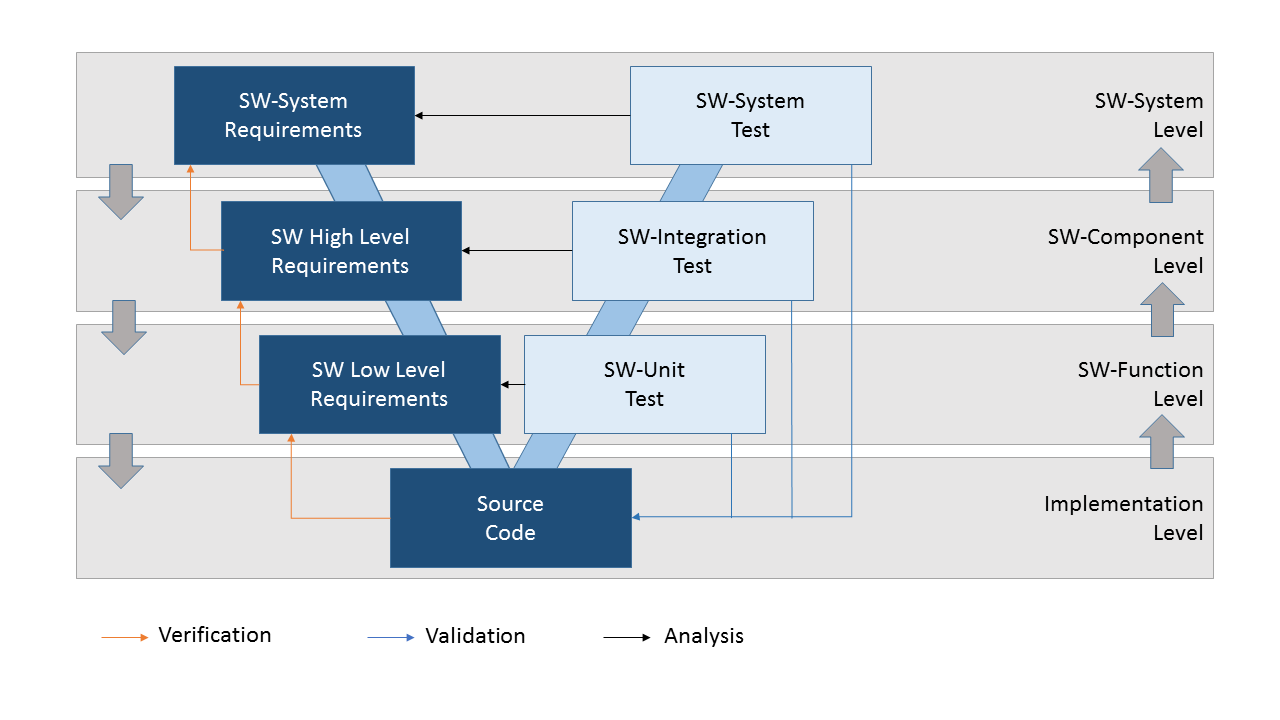
\includegraphics[width=14cm, height=14cm]{./images/V-Model}
\centering
\caption{V-Model}
\label{fig:v-model}
\end{figure}


\par To give small overview of V-model, it starts with requirement phase. Where customers and OEMs provide their product requirements. After that hardware and software architecture requirements are carried out and then process go to much more detail. In next phase component level requirements are collected and analyzed. After all high level and low level requirements, implementation process starts. After implementation, different testing techniques are performed at each corresponding phase, to identify bugs in low level, high level and system level design and implementation of product. And after all this final product is delivered to customer or OEMs.

\par Sequential development where software development waits for available hardware, is still prevailing industry norm. And this flaw of sequential development method is that to implementing software for product, hardware requirement must be known to software developers. Software developers need hardware architecture, memory, input/output(I/O) and many more parameter to design the architecture of software. After building the software for given hardware architecture and product, software tester need to test it on hardware and which should be available to testers. In some cases this hardware dependencies are observed and it delays the product release to customer, OEMs or to market. 

\subsection{Parallel development}
For every product development, time, cost and quality, these are key concerns. In device supply chain of semiconductor companies and OEMs are turning to parallel product development to shorten the development cycles and buy time to integrate  and test products. Virtual prototypes are used in parallel development, where virtual prototypes are functional software model of systems under development. These virtual prototypes are used in unavailability of harware, which helps faster software development. 

\begin{figure}[h!]
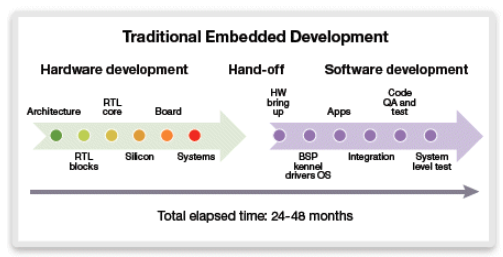
\includegraphics[width=12cm, height=7cm]{./images/seq_dev}
\centering
\caption{Time estimation for sequential product development}
\label{fig:seqn_dev}
\end{figure}

\par Embedded devices mostly depends upon custom hardware. These devices have broad array of use cases and hence they give rise to broad array of hardware architectures. There is no standardize platform is available. Absence of standardization increases  the time in product development. As mentioned in this [ref], realistic time estimation to develop complex embedded project requires 36 to 48 months of time with sequential development method.  12-18 months to hardware development, and 12-18 months for software development and 6-12 months for integration, verification and validation. Above figure\ref{fig:seqn_dev} illustrates the estimate time to build product using sequential method.

\par As we seen in above figure \ref{fig:seqn_dev}, software development lies on right hand side. And shifting left the software development process with parallel to hardware development results in parallel development. It can be seen in following figure \ref{fig:par_dev}. In parallel development, hardware and software team work in lock-step, communicating regularly, and continuously integrating hardware and software results into save time for modifications. With use virtual prototype tools parallel development of product can be possible. 

\begin{figure}[h!]
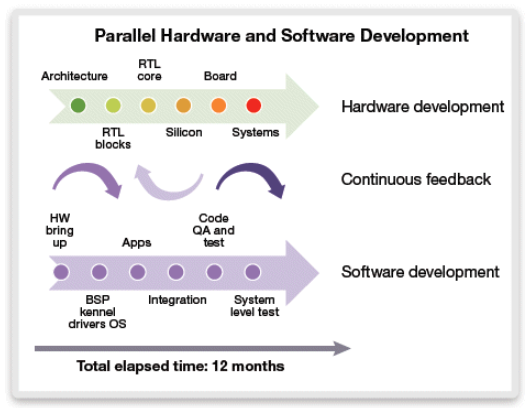
\includegraphics[width=12cm, height=10cm]{./images/par_dev}
\centering
\caption{Hardware and software development in parallel}
\label{fig:par_dev}
\end{figure}

\par In some scenarios, the system(s) on chip(SoC) takes time to come back from fabrication. In such scenarios, using virtual prototype of same SoC, software development can moves forward. It gives time to software developers for debugging and testing. With use of virtual prototypes in parallel development, avoid delays in product development as well as in product release in market. 

\section{Motivation}
Advanced risc machine(ARM), is family of reduced instruction set computing(RISC) architectures for computer processors. Arm holdings develops architecture and licenses it to other companies, who design their SoC product that includes architecture provided by ARM incorporate with memory, interfaces and many more. Processor architectures made by ARM are widely used automotive industry to develop ECUs as well as in other consumer industry for electronic products. ARM also provides the solutions for virtual prototyping, which provides motivation to my thesis work. Also it provide development solutions to embedded systems and servers. These tools are used in development od billions of ARm-based devices on the market.

\par As previously discussed how virtual prototypes help in early software development independent to physical availability of hardware. Goal of the ARM is to provide pre-silicon software development and analysis with better analysis, accuracy, availability, performance and ease of use. Following diagram \ref{fig:arm_dig1} illustrates available virtual prototypes/simulators from ARM with respect to abstraction level and simulation speed.

\begin{figure}[h!]
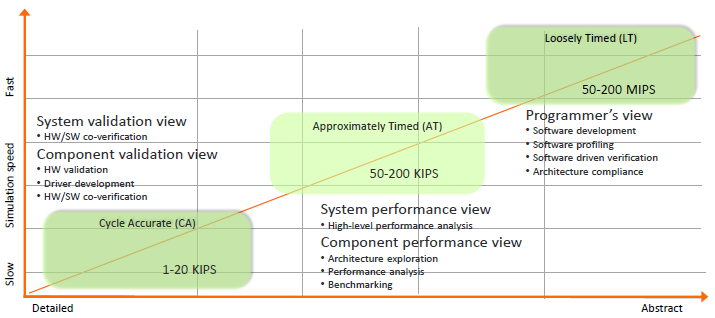
\includegraphics[width=14cm, height=10cm]{./images/arm_dig1}
\centering
\caption{ARM virtual prototype solutions}
\label{fig:arm_dig1}
\end{figure}

\par In above diagram \ref{fig:arm_dig1} ARM has cycle accurate tool which provides detailed abstraction level but slow simulation speed in between 1-20 kilo instructions per second(KIPS). This tool can be used for system validation and component validation applications such as hardware/software co-verification, hardware validation, driver development. This cycle accurate tool is known as ARM cycle models. ARM also provide loosely timed tool for simulation of SoCs. Which does not need detailed abstraction level and provides high simulation speed witn 50-200 million instructions per cycle(MIPS). This loosly coupled tool is known as ARM Fast Models. It can be used for application like software development, software profiling, and software driven verification.

\par Above diagram \ref{fig:arm_dig1} shows that for detailed abstraction level ARM cycle models can be applied but it provide slow simulation speed. Whereas ARM fast models can be applied where high simulation speed and not detailed abstraction level required. But there is no tool available where intermediate simulation speed and abstraction level required. For targeted application such as software profiling, benchmarking, performance analysis and software development. All these tools are expensive and also sometimes project dependent. And this problem motivates me to perform my research in my master thesis and find the optimal solution.

\par Performance of software, running on hardware can be measured.  Using machine learning it is possible to learn the performance relevant aspects of hardware platforms (SoC) to be able to predict the timing behavior of different applications. Performance of software running hardware can be measured in terms of micro-architectural events. Now a days every processor comes with hardware performance counter to monitor micro-architectural events. By running different software applications on two embedded cross platform hardware, statistical relationship can be formed and using this relationship can be use to predict the performance of software using machine learning. 

\subsection{Outline}





